\documentclass[11pt]{article}

\usepackage[margin=1in]{geometry}
\usepackage{amsmath,amssymb}
\usepackage{booktabs}
\usepackage{graphicx}
\usepackage{hyperref}
\usepackage{xcolor}

\newcommand{\linf}{\ell_\infty}
\newcommand{\ltwo}{\ell_2}
\newcommand{\epsinf}{\varepsilon_\infty}
\newcommand{\epstwo}{\varepsilon_2}

\title{Where Does Adversarial Vulnerability Come From?\\
A Controlled Gaussian Study with a Real-Data Check}
\author{}
\date{}

\begin{document}
\sloppy
\maketitle

\begin{abstract}
Why are accurate classifiers so easy to fool with tiny perturbations? We study
the smallest setting in which the question has an exact answer: Gaussian
inputs whose Bayes-optimal classifier is linear. There, the $\ell_\infty$
flip radius is $|\mathrm{LLR}|/\|w\|_1$ with $\|w\|_1=\sum_i d'_i/\sigma_i$, and
five synthetic experiments show that this quantity, not any single fragile feature,
explains what trained networks do. Vulnerability grows when
(i)~the same evidence is \emph{spread} over more dimensions
(radius $\propto k^{-1/2}$ in $\ell_\infty$, unchanged in $\ell_2$), and
(ii)~a feature's \emph{scale} (its class-mean gap) is small next to the budget,
which is Ilyas et al.'s notion of non-robustness. It does \emph{not} grow with
a feature's statistical reliability: at fixed scale, a $4\times$ more reliable
feature is no safer. A trained MLP matches the Bayes-optimal classifier's
vulnerability, so this is a property of the data and threat model, not of
training; no single weak dimension is fragile, only their sum; and
interventions that help do so by shrinking $\|w\|_1$ and pay in accuracy. A mixing test on MNIST (E6) confirms the geometry controls but not the $\sqrt k$ law: natural pixels are already near the saturated regime, and on CIFAR-10 the $\linf$ cost of using more directions comes from a shrinking $\ltwo$ margin, not from spread. We
state what would falsify the account, where it is weakest, and where we expect
readers to disagree.
\end{abstract}

\section{The question and the claim}

Ilyas et al.~\cite{ilyas2019} propose that adversarial examples exploit
\emph{non-robust features}: predictive, but brittle. Goodfellow et
al.~\cite{goodfellow2015} proposed earlier that the cause is linearity in high
dimension: a perturbation of size $\varepsilon$ in every coordinate moves a
linear score by $\varepsilon\|w\|_1$, which grows with dimension even when each
coordinate's change is imperceptible. These stories are usually told as
alternatives. We ask what a fully controlled example says about them.

\paragraph{Claim.} In a task where the optimal classifier is linear, $\linf$
vulnerability is set by $\|w\|_1=\sum_i d'_i/\sigma_i$: the evidence the
classifier collects per unit of absolute noise scale, summed over dimensions.
Two things make it large: evidence \emph{spread} over many dimensions, and
features of small \emph{scale} (class-mean gap $\Delta\mu_i$ small relative to
the budget $\varepsilon$), the operational meaning of ``non-robust'' in
\cite{ilyas2019}. A feature's statistical \emph{reliability} $d'$ is not a
cause. The trained network inherits all of this from the data; it is not a
learning failure.

\paragraph{What would falsify it.} The claim predicts five things, each of
which could have come out otherwise:

\begin{enumerate}
\item[\textbf{P1}] At fixed information, the minimal $\linf$ flip radius falls as
$k^{-1/2}$ in the number $k$ of dimensions sharing it, while the $\ltwo$ radius
is unchanged.
\item[\textbf{P2}] A trained MLP is no more vulnerable than the Bayes-optimal
classifier. If it were markedly worse, there would be learned fragility beyond
what the data imposes.
\item[\textbf{P3}] Each weak dimension, attacked alone, is \emph{harder} to flip
than the strong one. Only their sum is dangerous.
\item[\textbf{P4}] Interventions that raise robustness do so by lowering
$\|w\|_1$ and pay for it in accuracy; the exchange rate is set by the discarded
information.
\item[\textbf{P5}] For a single feature, the flip radius is proportional to its
scale $\Delta\mu$ and nearly independent of its reliability $d'$ at fixed
$\Delta\mu$. If reliability were the cause, a more reliable feature would be
safer.
\end{enumerate}

\paragraph{Terminology.} Two words are kept apart throughout. A dimension is
\emph{weak} if it is statistically unreliable on its own (small $d'$). It is
\emph{non-robust at budget $\varepsilon$} if its class-conditional correlation
does not survive the worst-case $\varepsilon$-perturbation, which for a Gaussian
feature means $\Delta\mu_i/2<\varepsilon$ (Ilyas et al.'s operational
definition, applied to our task). Both are fixed by the generative model
\emph{before} any attack is run, which avoids the circularity of calling
``non-robust'' whatever the attack succeeded through. In the task of
Table~\ref{tab:setup} the weak dimensions are also non-robust at $\varepsilon=0.3$
(half-gap $0.2<0.3$) and the strong one is neither, so Experiments~2--4 cannot
separate weakness from scale. Experiment~5 does.

\section{The mechanism in one equation}
\label{sec:mechanism}

Let $y\in\{0,1\}$ be balanced and, conditionally on $y$, let the inputs be
independent Gaussians
\[
x_i = \big(y-\tfrac12\big)\,\Delta\mu_i + \sigma_i\,\xi_i,\qquad \xi_i\sim\mathcal N(0,1),
\]
with per-dimension discriminability $d'_i=\Delta\mu_i/\sigma_i$. The inputs are
deliberately \emph{not} clipped to $[0,1]$: the Bayes rule is then exactly
linear and the budget is not confounded with the size of the domain. The
log-likelihood ratio is
\[
\mathrm{LLR}(x)=\sum_i w_i x_i,\qquad w_i=\frac{\Delta\mu_i}{\sigma_i^2},
\qquad \text{Bayes accuracy}=\Phi\!\Big(\tfrac12\sqrt{\textstyle\sum_i d_i'^2}\Big).
\]
The smallest perturbation that flips a correctly classified point is, by
duality of norms,
\begin{equation}
\epsinf(x)=\frac{|\mathrm{LLR}(x)|}{\|w\|_1},\qquad
\epstwo(x)=\frac{|\mathrm{LLR}(x)|}{\|w\|_2}.
\label{eq:mineps}
\end{equation}
Now spread a fixed amount of evidence $d'$ equally over $k$ dimensions with
the same noise level $\sigma$, so $d'_i=d'/\sqrt k$. Then $w_i=d'/(\sqrt k\sigma)$
and
\begin{equation}
\|w\|_2=\frac{d'}{\sigma}\ \ (\text{independent of }k),\qquad
\|w\|_1=\sqrt k\,\frac{d'}{\sigma}.
\label{eq:norms}
\end{equation}
The classifier's accuracy and $\ltwo$ margin are identical for every $k$; its
$\linf$ margin shrinks like $k^{-1/2}$. This is the whole mechanism: an $\linf$
ball lets the attacker move all $k$ coordinates by $\varepsilon$ in the
worst-case direction, while an $\ltwo$ ball of the same radius must share its
budget across them. Everything below tests whether this accounts for what
trained networks do.

\paragraph{Metric.} For each correctly classified test point we compute the
minimal flipping radius: exactly from~\eqref{eq:mineps} for the Bayes rule, and
by per-point bisection over a 20-step PGD attack for trained networks (we
verified that on the Bayes rule this agrees with~\eqref{eq:mineps} to within
the bisection tolerance, $2.4\times10^{-4}$). The empirical CDF of this radius
\emph{is} the attack-success-versus-$\varepsilon$ curve, so one number per point
replaces a grid of budgets. Models are one-hidden-layer MLPs (8 ReLU units,
Adam, 500 steps, weight decay $10^{-2}$) on 4{,}000 training points; all
results use 2{,}000 test points and 10 seeds, reported as mean $\pm$ standard
deviation over seeds of the per-seed median.

\begin{table}[h]
\centering
\caption{The task for Experiments 2--4: one strong dimension and five weak
ones. Single-dimension accuracy is $\Phi(d'/2)$. Together the five weak
dimensions have a larger total weight ($32.0$) than the strong one ($11.1$) and
slightly more squared discriminability ($12.8$ vs.\ $11.1$), yet individually
each is weak.}
\label{tab:setup}
\begin{tabular}{lccccc}
\toprule
Dimension & $\Delta\mu$ & $\sigma$ & $d'$ & single-dim.\ accuracy & Bayes weight $w_i$ \\
\midrule
strong ($x_0$) & 1.0 & 0.30 & 3.33 & 0.952 & 11.1 \\
weak ($x_1\ldots x_5$, each) & 0.4 & 0.25 & 1.60 & 0.788 & 6.4 \\
\midrule
all six, Bayes-optimal & & & 4.89 & 0.993 & $\|w\|_1=43.1,\ \|w\|_2=18.1$ \\
\bottomrule
\end{tabular}
\end{table}

\section{Experiments}

\subsection{E1. The same evidence, spread over more dimensions}

\textbf{Design.} Fix the total discriminability at $d'=1/0.3$ (Bayes accuracy
$95.2\%$) and split it equally over $k\in\{1,2,4,\ldots,64\}$ dimensions, each
with $\sigma=0.25$. Accuracy is the same at every $k$ by construction. Only the
\emph{number of places the evidence lives} changes. We train an MLP at each $k$
and compute the Bayes rule exactly.

\textbf{Result.} (Figure~\ref{fig:dims}, Table~\ref{tab:dims}.) The median
$\linf$ radius falls from $0.43$ at $k{=}1$ to $0.054$ at $k{=}64$, a log--log
slope of $-0.4995$ for the Bayes rule and $-0.4987$ for the MLP, against the
predicted $-0.5$. The median $\ltwo$ radius is constant ($0.43$ at every $k$,
slope $0.000$ and $-0.001$). The trained MLP lies on the exact curve at every
$k$, with seed-to-seed standard deviation at most $0.006$.

\begin{figure}[h]
\centering
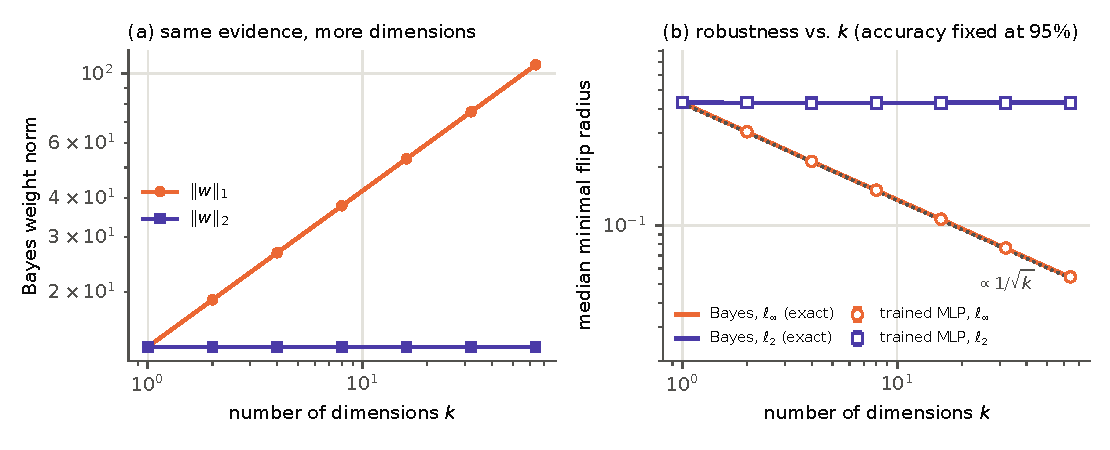
\includegraphics[width=0.98\textwidth]{fig_rc_dimensions.pdf}
\caption{E1. (a) At fixed total evidence, $\|w\|_2$ is constant and $\|w\|_1$
grows as $\sqrt k$ (Eq.~\ref{eq:norms}). (b) Median minimal flip radius versus
$k$: exact Bayes (lines) and trained MLP (markers, $\pm1$ s.d.\ over 10 seeds,
smaller than the markers for $\linf$). Accuracy is 95\% throughout.}
\label{fig:dims}
\end{figure}

\begin{table}[h]
\centering
\caption{E1 numbers. Median minimal flip radius; MLP: mean $\pm$ s.d.\ over 10
seeds. Bayes values are exact, averaged over test sets.}
\label{tab:dims}
\begin{tabular}{rcccccc}
\toprule
$k$ & $\|w\|_1/\|w\|_2$ & Bayes $\epsinf$ & MLP $\epsinf$ & Bayes $\epstwo$ & MLP $\epstwo$ & MLP acc.\\
\midrule
1  & 1.00 & 0.432 & 0.433$\pm$0.006 & 0.432 & 0.433$\pm$0.006 & 0.951$\pm$0.004\\
4  & 2.00 & 0.214 & 0.215$\pm$0.003 & 0.429 & 0.429$\pm$0.006 & 0.955$\pm$0.005\\
16 & 4.00 & 0.108 & 0.108$\pm$0.002 & 0.432 & 0.430$\pm$0.007 & 0.953$\pm$0.004\\
64 & 8.00 & 0.054 & 0.054$\pm$0.001 & 0.432 & 0.429$\pm$0.007 & 0.950$\pm$0.005\\
\bottomrule
\end{tabular}
\end{table}

\textbf{Reading.} \textbf{P1 holds.} A classifier can lose a factor of eight in
$\linf$ robustness, with no change in accuracy, no change in $\ltwo$
robustness, and no individually fragile feature, purely because its evidence
is divided among more coordinates. The ratio $\epstwo/\epsinf$ equals
$\|w\|_1/\|w\|_2$ at every $k$.

\subsection{E2. The optimal classifier is as vulnerable as the trained one}

\textbf{Design.} Use the task of Table~\ref{tab:setup}. Attack the trained MLP
and the exact Bayes-optimal classifier. The Bayes classifier has no
optimisation, no overfitting and no inductive bias.

\textbf{Result.} (Figure~\ref{fig:ecdf}.) The two curves nearly coincide. Median
$\epsinf$ is $0.277\pm0.002$ (Bayes) versus $0.285\pm0.002$ (MLP); the fraction
of points flipped at $\varepsilon=0.3$ is $58.1\%$ versus $55.3\%$. Clean
accuracy is $0.9926$ versus $0.9924\pm0.0014$. If anything, the trained
network is slightly \emph{more} robust than the optimum.

\begin{figure}[h]
\centering
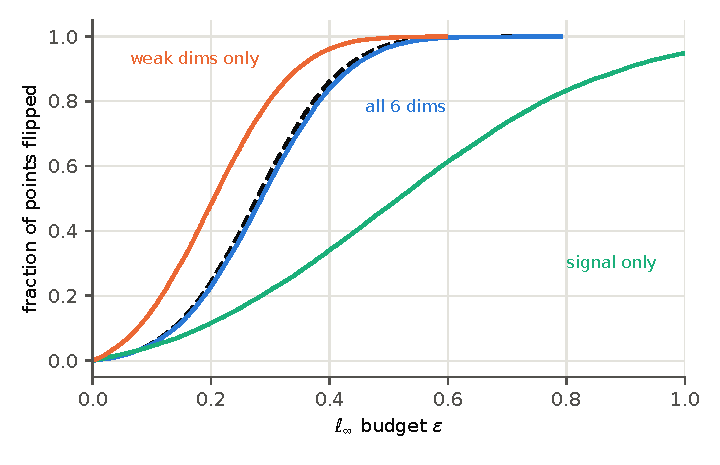
\includegraphics[width=0.62\textwidth]{fig_rc_ecdf.pdf}
\caption{E2 and E4. Fraction of test points flipped by an $\linf$ attack of
budget $\varepsilon$ (pooled over seeds). Dashed black: exact Bayes-optimal
classifier on all six dimensions; it lies on top of the trained MLP (blue).
Models restricted to the weak dimensions only (orange) or the strong one only
(green) are shown for comparison (E4).}
\label{fig:ecdf}
\end{figure}

\textbf{Reading.} \textbf{P2 holds.} For this task, the vulnerability
is a property of \emph{the data and the threat model}, not of how the network
was trained. This is also why the companion note's observation~\cite{earlier} that the MLP
relies on the weak dimensions \emph{less} than a Bayes-optimal classifier does
is consistent with its being vulnerable: the weights the optimum places there are already
enough.

\subsection{E3. Who is vulnerable? No dimension is; the sum is}

\textbf{Design.} Restrict the attacker to a subset of coordinates and measure
$\epsinf$ for the Bayes rule and the MLP, again on Table~\ref{tab:setup}'s task.
This is the control missing from the usual ``attack only the weak features''
experiment, which compares five dimensions to one and so confounds feature
type with attack dimensionality.

\begin{table}[h]
\centering
\caption{E3. $\linf$ attack restricted to a subset $S$ of dimensions: median
minimal flip radius (larger = harder) and fraction flipped at $\varepsilon=0.3$.
For the Bayes rule $\epsinf=|\mathrm{LLR}|/\|w_S\|_1$ exactly.}
\label{tab:subsets}
\begin{tabular}{lccccc}
\toprule
Attacked dims $S$ & $\|w_S\|_1$ & Bayes $\epsinf$ & MLP $\epsinf$ & Bayes flipped & MLP flipped\\
\midrule
strong dimension (1) & 11.1 & 1.076 & 1.012$\pm$0.018 & 3.3\% & 3.8\%\\
\emph{one} weak dimension & 6.4 & 1.868 & 2.005$\pm$0.078 & 1.3\% & 1.3\%\\
all 5 weak dimensions & 32.0 & 0.374 & 0.397$\pm$0.006 & 31.1\% & 27.3\%\\
all 6 dimensions & 43.1 & 0.277 & 0.285$\pm$0.002 & 58.1\% & 55.3\%\\
\bottomrule
\end{tabular}
\end{table}

\begin{figure}[h]
\centering
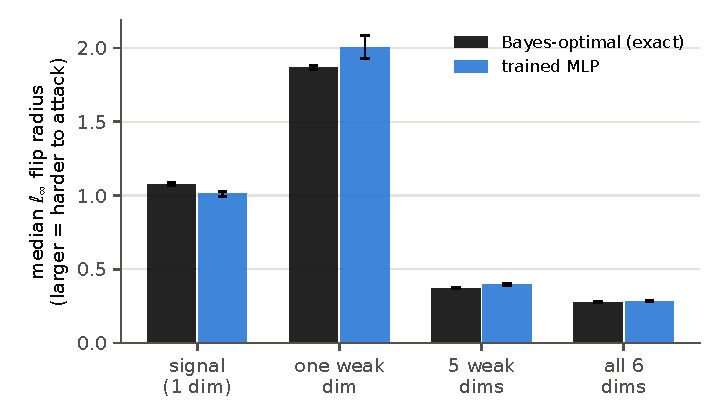
\includegraphics[width=0.62\textwidth]{fig_rc_subsets.pdf}
\caption{E3. Median $\linf$ flip radius when the attacker controls only the
listed dimensions. One weak dimension is the \emph{hardest} to exploit; five
together are about three times easier than the strong dimension alone.}
\label{fig:subsets}
\end{figure}

\textbf{Reading.} \textbf{P3 holds.} A single weak dimension is harder to flip
than the strong one ($1.87$ vs.\ $1.08$): its weight is smaller. The five
together are $\approx 3\times$ easier to flip than the strong one ($0.37$ vs.\
$1.08$) because $\|w_S\|_1$ adds up ($32.0$ vs.\ $11.1$). The vulnerability is
therefore not located in any feature. This corrects the common summary that
``attacks on the weak features are more effective'': per dimension they are
less effective, per attacker they are more, simply because there are more of
them.

\subsection{E4. Interventions work by shrinking $\|w\|_1$, and pay in accuracy}

\textbf{Design.} Compare: all six dimensions; the strong dimension only
(removing the weak dimensions from the input); the five weak dimensions only
(the converse); and all six with a first-layer
$L_1$ penalty $\lambda\in\{0.02,\dots,0.2\}$ pushing weights onto fewer
dimensions. Report $\linf$ and $\ltwo$ radii.

\begin{table}[h]
\centering
\caption{E4. Clean accuracy and median minimal flip radius (mean $\pm$ s.d.\ over
10 seeds). The Bayes-optimal rule on the same inputs gives $\epsinf=0.517$ (strong only),
$0.204$ (weak only) and $0.277$ (all six).}
\label{tab:interv}
\begin{tabular}{lcccc}
\toprule
Model & accuracy & $\epsinf$ & $\epstwo$ & $\|w\|_1/\|w\|_2$ (Bayes)\\
\midrule
all six (MLP)            & 0.992$\pm$0.001 & 0.285$\pm$0.002 & 0.666$\pm$0.004 & 2.38\\
strong only              & 0.953$\pm$0.005 & 0.517$\pm$0.006 & 0.517$\pm$0.006 & 1.00\\
weak only (5 dims)       & 0.962$\pm$0.003 & 0.205$\pm$0.002 & 0.458$\pm$0.004 & 2.24\\
all six, $L_1$ $\lambda=0.05$ & 0.987$\pm$0.002 & 0.343$\pm$0.005 & 0.651$\pm$0.006 & --\\
all six, $L_1$ $\lambda=0.10$ & 0.976$\pm$0.004 & 0.402$\pm$0.010 & 0.598$\pm$0.011 & --\\
all six, $L_1$ $\lambda=0.20$ & 0.957$\pm$0.005 & 0.496$\pm$0.010 & 0.529$\pm$0.006 & --\\
\bottomrule
\end{tabular}
\end{table}

\begin{figure}[h]
\centering
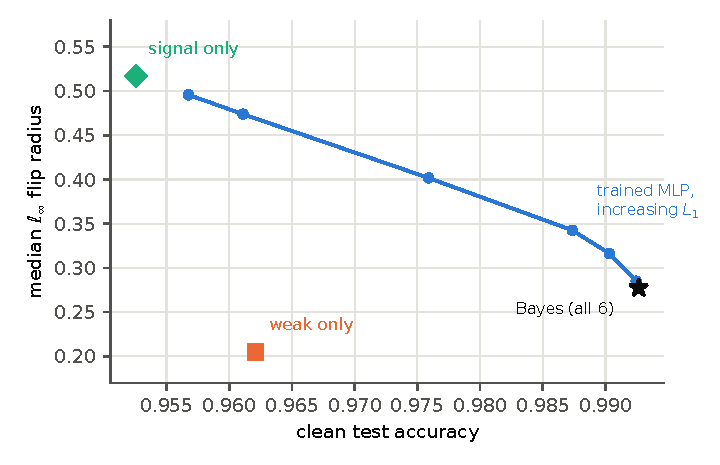
\includegraphics[width=0.62\textwidth]{fig_rc_tradeoff.pdf}
\caption{E4. Accuracy versus $\linf$ robustness. Increasing the $L_1$ penalty
(blue) moves the model from the Bayes-optimal point (star) toward the
strong-only solution (green diamond). The weak-only model (orange) is both
more accurate than strong-only and far less robust.}
\label{fig:tradeoff}
\end{figure}

\textbf{Result.} Three observations. (i)~Removing the weak dimensions raises
$\epsinf$ from $0.285$ to $0.517$ ($1.8\times$) and costs $4.0$ points of
accuracy. (ii)~The weak-only model is the instructive control: at $96.2\%$
accuracy ($>$ strong-only) it is $2.5\times$ \emph{less} $\linf$-robust. Which
dimensions you keep matters less than how many share the evidence. Its
$\ltwo$ radius ($0.458$) is close to the strong-only model's ($0.517$), and
$\epstwo/\epsinf=2.23$ matches $\|w\|_1/\|w\|_2=\sqrt5$ as predicted.
(iii)~The $L_1$ sweep walks close to a line from the Bayes point to the
strong-only point: $\linf$ radius rises $74\%$ while accuracy falls $3.6$
points. Along it the $\ltwo$ radius \emph{falls} ($0.666\to0.529$): the
penalty concentrates weight, which reduces $\|w\|_1$ at fixed $\|w\|_2$ and
trades one kind of robustness for accuracy rather than creating robustness
outright.

\textbf{Reading.} \textbf{P4 holds.} Robustness gained by sparsifying is paid
for with the evidence discarded; nothing in these runs offers a free lunch.
Note what this does \emph{not} show: that a smarter regulariser or architecture
could not do better on real data. It shows that, here, the exchange is set by
the data.

\subsection{E5. Scale, not reliability: one feature, two knobs}

\textbf{Design.} Everything so far moved weak features and strong features
together. Here we pull the two apart in the simplest possible case: a single
Gaussian feature with class-mean gap $\Delta\mu\in\{0.05,\dots,0.8\}$ and
reliability $d'\in\{1.5,3,6\}$, with $\sigma=\Delta\mu/d'$. Reliability sets
accuracy ($0.77,\ 0.93,\ 0.999$); scale sets robustness in Ilyas et al.'s sense.
Trained models carry a fixed standardisation layer so that tiny-scale inputs are
not handicapped by the optimiser; attacks act on raw inputs.

\textbf{Result.} (Figure~\ref{fig:scale}, Table~\ref{tab:scale}.) The median
flip radius is proportional to $\Delta\mu$ across a $16\times$ range, with a
constant $\epsinf/\Delta\mu=0.69$, $0.53$, $0.50$ for $d'=1.5,3,6$ (to two
digits at every scale). A $4\times$ change in reliability changes the radius by
$1.4\times$, in the wrong direction for a reliability explanation: the
\emph{more} reliable feature is slightly \emph{less} robust, approaching the
limit $\Delta\mu/2$ (in one dimension the flip radius is just the distance
to the decision boundary). The trained MLP matches the exact Bayes radius to
within $0.0011$ in every cell.

\begin{figure}[h]
\centering
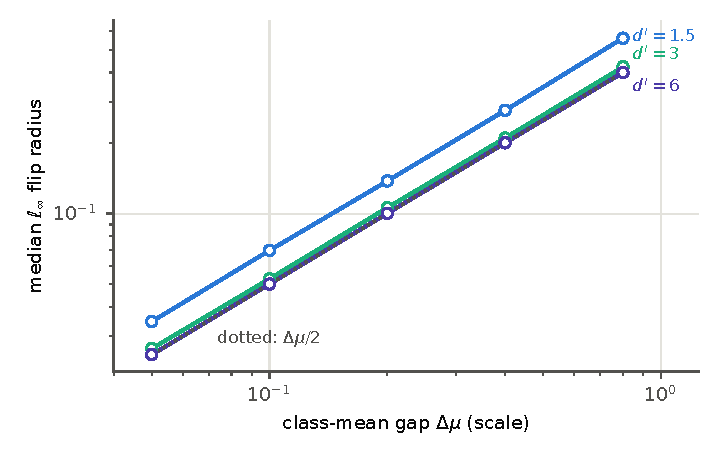
\includegraphics[width=0.62\textwidth]{fig_rc_scale.pdf}
\caption{E5. Median $\linf$ flip radius of a single-feature classifier versus
its class-mean gap $\Delta\mu$, at three reliabilities. Lines: exact Bayes;
markers: trained MLP ($\pm1$ s.d., 10 seeds). Radius tracks scale; reliability
only shifts the line by a factor of at most $1.4$.}
\label{fig:scale}
\end{figure}

\begin{table}[h]
\centering
\caption{E5. Median $\linf$ flip radius (exact Bayes; MLP within $0.0011$) and,
in parentheses, the ratio $\epsinf/\Delta\mu$, which depends on $d'$ alone.}
\label{tab:scale}
\begin{tabular}{lccc}
\toprule
$\Delta\mu$ & $d'=1.5$ (acc.\ 0.77) & $d'=3$ (acc.\ 0.93) & $d'=6$ (acc.\ 0.999)\\
\midrule
0.05 & 0.035 (0.69) & 0.027 (0.53) & 0.025 (0.50)\\
0.1  & 0.070 (0.70) & 0.053 (0.53) & 0.050 (0.50)\\
0.2  & 0.138 (0.69) & 0.106 (0.53) & 0.100 (0.50)\\
0.4  & 0.276 (0.69) & 0.210 (0.53) & 0.200 (0.50)\\
0.8  & 0.560 (0.70) & 0.422 (0.53) & 0.400 (0.50)\\
\bottomrule
\end{tabular}
\end{table}

\textbf{Reading.} \textbf{P5 holds.} A single, nearly perfectly reliable
feature ($d'=6$, $99.9\%$ accuracy) of small scale is as attackable as a
radius of $\Delta\mu/2$ allows: at $\Delta\mu=0.05$ it flips at
$\varepsilon=0.025$. This is what ``non-robust'' means in \cite{ilyas2019},
and it is a different knob from E1's spread. Both enter the same formula,
$\|w\|_1=\sum_i d'_i/\sigma_i$: E1 grows it through the number of terms, E5
through a smaller $\sigma_i$ at fixed $d'_i$. A caution on E1: there each
dimension's $\Delta\mu_k=d'\sigma/\sqrt k$ shrinks with $k$ as well, so E1 alone
does not show that spread is separate from scale. What separates them is the
$\ltwo$ control: if per-coordinate scale were the cause, the $\ltwo$ radius would
move with $k$ too, and it does not.

\section{Does it survive on real data? E6}

\textbf{Design.} We test the spread mechanism on MNIST by changing only how widely
information is spread across coordinates. Inputs (centred, unclipped) are mixed
by a fixed block-diagonal random orthogonal matrix $Q_k$ with block size
$k\in\{1,4,16,49,196,784\}$ over a random pixel permutation. $Q_k$ preserves
information and $\ltwo$ geometry exactly; only the coordinate basis changes. An MLP
(784--256--10, SGD with momentum and $\ell_2$ weight decay, which are rotation-equivariant;
Adam is not) is trained and attacked in the mixed coordinates with the same minimal-radius metric
(10{,}000 training and 1{,}000 test points, 5 seeds), on 3-vs-7 and on all ten classes.
Predictions: accuracy and $\epstwo$ flat in $k$; $\epsinf$ falling as $k^{-1/2}$.

\begin{table}[h]
\centering
\caption{E6. MNIST, median minimal flip radius, mean over 5 seeds
(s.d.\ in text). The last column is $\epstwo/\epsinf$; a dense isotropic direction
gives $\sqrt{2/\pi}\sqrt{784}=22.3$.}
\label{tab:real}
\begin{tabular}{llccccc}
\toprule
Task & $k$ & accuracy & $\epsinf$ & $\epstwo$ & $\epstwo/\epsinf$\\
\midrule
3 vs.\ 7 & 1   & 0.991 & 0.0687 & 1.351 & 19.7\\
         & 16  & 0.991 & 0.0617 & 1.354 & 22.0\\
         & 196 & 0.991 & 0.0607 & 1.358 & 22.4\\
         & 784 & 0.991 & 0.0605 & 1.352 & 22.4\\
10 class & 1   & 0.956 & 0.0481 & 0.929 & 19.3\\
         & 16  & 0.957 & 0.0421 & 0.919 & 21.8\\
         & 196 & 0.955 & 0.0416 & 0.927 & 22.3\\
         & 784 & 0.956 & 0.0413 & 0.925 & 22.4\\
\bottomrule
\end{tabular}
\end{table}

\textbf{Result.} The controls hold: accuracy and $\epstwo$ do not change with $k$
(accuracy within $0.001$; $\epstwo$ within seed noise, s.d.\ $0.02$--$0.04$). The
$\linf$ prediction \emph{fails as stated}: $\epsinf$ falls by only $12\%$
(3-vs-7) and $14\%$ (ten classes) between $k{=}1$ and $k{=}784$, not by the factor of
$28$ that $k^{-1/2}$ would give. The cause is visible in the last column: $\epstwo/\epsinf$,
the trained network's analogue of $\|w\|_1/\|w\|_2$, is already $19$--$20$ in the pixel
basis and saturates at $22.4$, the value for a dense isotropic direction. Equation~\eqref{eq:mineps}
still organises the data: the radius is set by the $\ell_1$-to-$\ell_2$ ratio of the
classifier's gradient. But MNIST in its natural basis is already in the saturated regime, so
the spread knob of E1 has little room left to turn. We read this as a limit
on the claim: the $\sqrt k$ law describes how vulnerability grows with
spread, not that natural images are far from saturation, and E6 does not show the
latter either way. Mixing is a change of basis, not a new dataset.

\paragraph{E6b. CIFAR-10, number of directions used.} A second real-data check
varies how many input directions the network may use. A five-layer CNN (20{,}000
training and 500 test points, 5 seeds, SGD) sees only the projection of the
image onto the top-$m$ PCA directions; the attacker perturbs raw pixels with an
unclipped $\linf$ or $\ltwo$ ball, so only the in-subspace component matters.

\begin{table}[h]
\centering
\caption{E6b. CIFAR-10, median minimal flip radius over correctly classified points
(mean over 5 seeds). A dense isotropic direction gives $\epstwo/\epsinf=44.2$.}
\label{tab:cifar}
\begin{tabular}{rcccc}
\toprule
$m$ & accuracy & $\epsinf$ & $\epstwo$ & $\epstwo/\epsinf$\\
\midrule
16   & 0.442 & 0.0176 & 0.779 & 44.3\\
64   & 0.574 & 0.0102 & 0.431 & 42.2\\
256  & 0.704 & 0.0057 & 0.230 & 40.6\\
1024 & 0.780 & 0.0030 & 0.116 & 39.1\\
3072 & 0.778 & 0.0026 & 0.099 & 38.5\\
\bottomrule
\end{tabular}
\end{table}

Using more directions buys accuracy ($0.44\to0.78$) and costs $\linf$ robustness by
a factor of $6.8$, which is the exchange of P4 on real data. But the mechanism is not
spread: $\epstwo/\epsinf$ is near its dense limit at every $m$ and
\emph{decreases} slightly with $m$, while $\epstwo$ itself falls by
$7.9\times$. The $\linf$ loss is therefore almost entirely a shrinking $\ltwo$
margin, i.e.\ the network relies on lower-variance, smaller-margin directions
(the scale route of E5, not the spread route of E1). Caveat: medians are over
correctly classified points, so low-$m$ models are evaluated on an easier subset,
which overstates their robustness.

\paragraph{Earlier image result.} The companion note~\cite{earlier} reports that a
background-only attack flips $67\%$ of predictions at $\varepsilon=0.3$ (FGSM) on a
circle-vs-square task, and that a two-branch CNN reduces this to $31\%$. That used a
different metric, has not been re-run here, and we do not rely on it.

\section{Discussion: what this does and does not say}

\paragraph{Relation to non-robust features.} The answer to ``do non-robust
features cause vulnerability?'' is yes, with two qualifications. First,
non-robust must be read as Ilyas et al.\ define it, small class separation
relative to the budget (scale, E5), and not as ``statistically weak'': a
nearly perfect small-scale feature is the most attackable thing in this paper.
Second, the vulnerable direction in the six-dimension task is made of
statistically \emph{legitimate} features: the Bayes classifier wants them, and
the five weak dimensions together have $2.9\times$ the weight $\|w_S\|_1$ of the
strong one (and $1.15\times$ its squared discriminability). A coalition of small contributions is easy to move, which is the spread
effect (E1, E3). We do not claim this is the whole of Ilyas et al.'s account on
natural images, where non-robust features also have a frequency character
that this toy does not model.

\paragraph{Relation to prior work.} The ingredients are not new: the
$\varepsilon\|w\|_1$ growth of linear scores is Goodfellow et
al.'s~\cite{goodfellow2015} linearity argument, with $\ell_1$-gradient norms
and input dimension linked in~\cite{simongabriel2019}; Gaussian
class-conditional models with one strong and many weak features appear
in~\cite{tsipras2018,schmidt2018}. What is added here is the isolation:
information held \emph{fixed}, only its spread varied, with exact predictions
checked against trained networks and against the Bayes rule, and a norm-swap
control ($\ltwo$ unchanged) that distinguishes accumulation from fragility,
and a factorial (E5) that separates a feature's scale from its reliability.

\paragraph{Where you may disagree.}
\begin{itemize}
\item \emph{``The task is linear, so of course.''} Yes, by design: it is the
case where the claim can be derived rather than argued. That a one-hidden-layer
MLP lands on the linear solution (E1, E2) shows the claim holds for a network
here, not that deep networks on natural data share it.
\item \emph{``$\linf$ is a convention, not a fact.''} Agreed, and the result
says so: under $\ltwo$ the same classifiers are indistinguishable across $k$.
The vulnerability is a statement about the pairing of a data distribution with
a threat model.
\item \emph{``Independent features are unrealistic.''} Correlated weak
features share noise and so carry less independent evidence; that would
weaken the effective $k$, not remove the mechanism. We have not tested it.
\item \emph{``Robust training obviously fixes this.''} It may, and adversarial
training is known to. Nothing here concerns whether it \emph{costs} what this
account predicts on real data.
\end{itemize}

\paragraph{Limitations.} One task family, equal-weight Gaussian dimensions,
a single small architecture, standardised inputs for E5 (without which a
tiny-scale feature is harder to train, itself a possible real-world factor),
PGD-based radii for trained models, and, on real data, only an MLP on MNIST in a rotated basis (E6). The strongest next test is
a trained deep network on a dataset where the number of dimensions
carrying a fixed amount of evidence can be varied in the native basis.

\appendix
\section{Reproducibility and relation to the earlier note}

All experiments are in \texttt{root\_cause\_experiments.py}, E5 in \texttt{root\_cause\_factorial.py}, E6 in \texttt{root\_cause\_realdata.py}, E6b in \texttt{root\_cause\_cifar.py}, and all figures and
numbers in \texttt{root\_cause\_figures.py}; E1--E5 take about seven minutes
on CPU and E6 and E6b about ten minutes each on one GPU. Training for E1--E5: Adam, learning rate $0.02$, 500 full-batch steps, weight decay
$10^{-2}$, 4{,}000 training and 2{,}000 test points, seeds $0$--$9$ reseeding
both data and initialisation. Minimal radii: bisection (14 iterations, search
range $[0,4]$) over 20-step PGD with step $\varepsilon/4$, counting a point as
flipped if \emph{any} iterate is misclassified; $\ltwo$ attacks use normalised
gradient steps with projection onto the ball.

\paragraph{What changed from the earlier note \cite{earlier}.}
(a)~Inputs are unclipped, which removes the $\varepsilon=0.5$ artifact and
makes the Bayes rule exactly linear. (b)~The metric is the minimal flip radius,
not success on a grid. (c)~The earlier headline that ``non-robust-only attacks
are $2$--$4\times$ more effective than robust-only attacks'' is replaced by
E3, which shows the comparison reflects five attackable dimensions versus
one. (d)~The earlier claim that removing the weak dimensions makes the model
``substantially harder to fool at every budget from $\varepsilon=0.05$'' was
too strong: in that note's own Table~2 the two models are no different below
$\varepsilon=0.10$ (B is slightly \emph{worse} at $0.05$). The gain appears at
larger budgets, consistent with the median radius of $0.28$ found here. (e)~Material
on activation sparsity, Model~C initialisation, pruning, and seed-dependent
collapse is not needed for the claim and is omitted.

\begin{thebibliography}{9}

\bibitem{earlier}
Companion note: \emph{Robust and Non-Robust Features in a Fully Controlled
Synthetic Classification Task: A Minimal Demonstration}
(\texttt{toy\_robust\_features\_paper.tex}, this repository).

\bibitem{goodfellow2015}
I.~Goodfellow, J.~Shlens, C.~Szegedy.
\emph{Explaining and Harnessing Adversarial Examples}. ICLR, 2015.

\bibitem{ilyas2019}
A.~Ilyas, S.~Santurkar, D.~Tsipras, L.~Engstrom, B.~Tran, A.~Madry.
\emph{Adversarial Examples Are Not Bugs, They Are Features}. NeurIPS, 2019.

\bibitem{tsipras2018}
D.~Tsipras, S.~Santurkar, L.~Engstrom, A.~Turner, A.~Madry.
\emph{Robustness May Be at Odds with Accuracy}. ICLR, 2019.

\bibitem{schmidt2018}
L.~Schmidt, S.~Santurkar, D.~Tsipras, K.~Talwar, A.~Madry.
\emph{Adversarially Robust Generalization Requires More Data}. NeurIPS, 2018.

\bibitem{simongabriel2019}
C.-J.~Simon-Gabriel, Y.~Ollivier, L.~Bottou, B.~Sch\"olkopf, D.~Lopez-Paz.
\emph{First-order Adversarial Vulnerability of Neural Networks and Input
Dimension}. ICML, 2019.

\end{thebibliography}

\end{document}
